\documentclass[titlepage, 11pt, reqno]{article}    % use "amsart" instead of "article" for AMSLaTeX format
\usepackage{my_packages}
\usepackage{tikz_packages}
\usepackage[american,siunitx]{circuitikz}
\usepackage{pgfplots}
\pgfplotsset{compat=newest}
\usepackage[explicit]{titlesec}
\usepackage{pdfpages}
% change the formatting for a section (which we're treating as a problem)
\titleformat{\section}[runin]{\normalfont\bfseries}{}{0em}{#1\ \thesection}
\crefformat{section}{problem #2#1#3}
\Crefformat{section}{Problem #2#1#3}


\begin{document}
\begin{titlepage}
    \centering
    \vspace{1cm}
    {\Large Spring 2017 MAE3134: Final Exam\par }
    \vspace{3cm}
    {11 May 2017\par}
    \vspace{1cm}
    \textbf{Resources allowed}: Open notes/book, calculator, ruler. 
    No computers or mobile devices.

    \vspace{1cm}
    {Name: \underline{\hspace{5cm}} \hspace{2cm} GWID:\underline{\hspace{5cm}}\par}
    \vspace{3cm}

    \begin{tabular}{|c|c|c|c|c|c|c|c|c|}
        \hline
        Prob. 1 & Prob. 2 & Prob. 3 & Prob. 4 & Prob. 5 & Prob. 6 & Prob. 7 & Prob. 8 & Total \\
        \hline
         & & & & & & & &\\[4ex]
        \hline
        10 & 5 & 20 & 20 & 10 & 5 & 10 & 20 & 100 \\[4ex]
        \hline
    \end{tabular}
    \vfill
\end{titlepage}

\section{Problem}\label{prob:sys_response_to_poles}
Elon Musk, CEO of SpaceX and Tesla Motors, has a background in physics but unfortunately has never passed a Linear Dynamics course. 
His newest space vehicle must satisfy the following second order time response specifications for a unit step input:
\begin{itemize}
    \item Percent Overshoot must be less than \(5 \%\),
    \item Peak time less than \SI{1}{\second},
    \item Settling Time less than \SI{5}{\second}.
\end{itemize}
Elon needs your help to choose a set of poles which will satisfy the specifications and save humanity from impending disaster.
\begin{enumerate}
    \item On the s-plane, or complex plane, map out the acceptable regions where you could locate poles and meet the requirements. 
    \item Label the specifications lines and show your work.
    \item Choose a set of poles that will meet the requirements.
    \item Determine the transfer function representation for this sytem.
    \item Use the initial and final value theorems to determine the initial and final values of \( x (t) \).
\end{enumerate}

\begin{figure*}[htbp]
\centering
\begin{scaletikzpicturetowidth}{0.95\textwidth}
    \begin{tikzpicture}[scale=\tikzscale]
        \draw[help lines, color=gray!50, dashed] (-8, -5) grid (8, 5);
        \draw[->, ultra thick] (-8, 0)--(8, 0) node[right]{Real};
        \draw[->, ultra thick] (0, -5)--(0, 5) node[above]{Imag};
    \end{tikzpicture}
\end{scaletikzpicturetowidth}
\end{figure*}

\newpage
\thispagestyle{plain}
\mbox{}


\section{Problem}
Given the state space representation defined as
\begin{align*}
    \vb{\dot{x}} &= A \vb{x} + B \vb{u}, \\
    \vb{y} &= C \vb{x} + D\vb{u},
\end{align*}
\textbf{DERIVE} the expression for the transfer function \(\frac{\vb{Y}(s)}{\vb{U}(s)}\).
\vspace{13cm}
\section{Problem}

List at least two advantages of state-space or ``modern control'' techniques as compared to ``classical control'' approaches.
\vspace{5cm}
\clearpage
\section{Problem}

For the electrical system in~\cref{fig:elec_circuit_2}:
\begin{enumerate}
    \item Find the differential equations of motion for the system.
    \item Find the state space representation of the system with your state vector defined as
        \begin{align*}
        \vb{x} = \begin{bmatrix}q_1 & i_1 & q_2 & i_2\end{bmatrix}^T,
        \end{align*}
        where \(q_1, i_1\) represent the charge and current in the left loop while \(q_2, i_2\) represent the charge and current in the right loop. 
        The output is defined as
        \begin{align*}
        y = \begin{bmatrix} q_1 & q_2 \end{bmatrix}^T.
        \end{align*}
\end{enumerate}
\begin{figure}[htbp]
\centering
\begin{scaletikzpicturetowidth}{0.8\textwidth}
    \begin{tikzpicture}[scale=\tikzscale]
        \draw (0,0) to[american voltage source,v<=\( u(t)\)] (0,2) 
        to[resistor, l^=$R_1$] (2,2) to[capacitor, l=$C$] (2,0) 
        to[inductor, l^=$L_1$] (0,0); 
        \draw (2,2) to[short] (4,2)
        to[inductor, l=$L_2$] (4,0) to[short] (2,0);
    \end{tikzpicture}
\end{scaletikzpicturetowidth}
\caption{Electrical Circuit~\label{fig:elec_circuit_2}}
\end{figure}
\clearpage
\newpage
\mbox{}
\clearpage
\section{Problem}
Consider the electrical circuit shown in~\cref{fig:elec_circuit}:
\begin{enumerate}
    \item Find the differential equations which govern the behavior of the electrical system.
    \item Construct the state space representation of the system. 
        Assume the desired output is the charge in the system.
    \item Find the output response of the system assuming zero initial conditions and a step input of \(u(t) = \SI{24}{\volt}\)
\end{enumerate}
\begin{figure}[htbp]
\centering
\begin{scaletikzpicturetowidth}{0.5\textwidth}
    \begin{tikzpicture}[scale=\tikzscale]
        \draw (0,0) to[american voltage source,v<=\( u(t)\)] (0,2) 
        to[inductor, l^=1<\henry>] (2,2) to[resistor, l=3<\ohm>] (2,0) 
        to[capacitor, l^=0.5<\farad>] (0,0); 
    \end{tikzpicture}
\end{scaletikzpicturetowidth}
\caption{Electrical Circuit~\label{fig:elec_circuit}}
\end{figure}
\clearpage
\newpage
\thispagestyle{plain}
\mbox{}
\clearpage
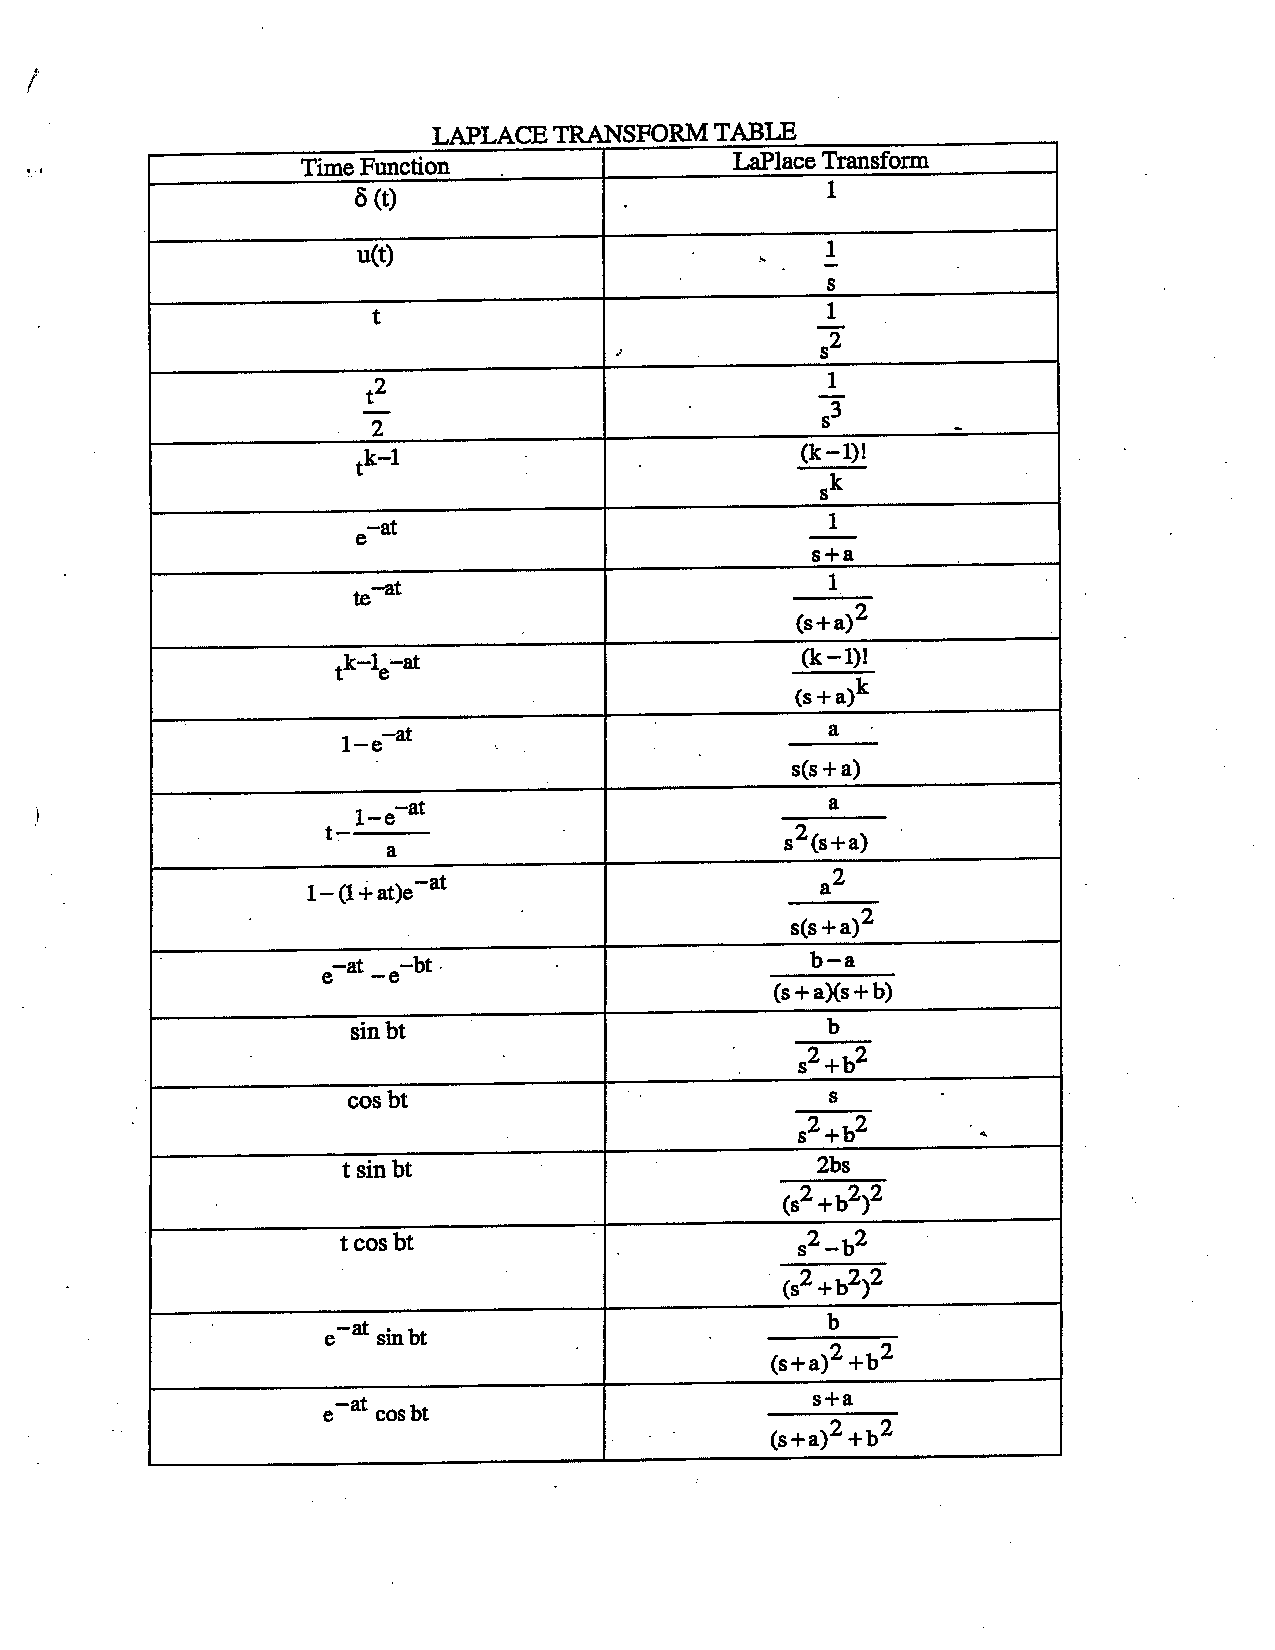
\includepdf{../../laplace_transform_table.pdf}
\end{document}  
